\documentclass[xcolor={dvipsnames}]{beamer}

\usetheme{CambridgeUS}

\definecolor{redUnipd}{HTML}{9b0014}
\definecolor{grayUnipd}{HTML}{444F51}
%Here the two main colors for the graphs:
\definecolor{lightred}{RGB}{255, 179, 178}
\definecolor{lightgrey}{RGB}{218, 218, 218}

\definecolor{myblue}{HTML}{317a9b}
%\definecolor{Black}{RGB}{0,62,114}
\newcommand{\bbf}[1]{\textcolor{black}{\bf #1}}
\newcommand{\rbf}[1]{\textcolor{redUnipd}{ #1}}
\usefonttheme{structurebold}
%\usecolortheme[named=myblue]{structure}
\setbeamercolor{structure}{fg=redUnipd}
%setbeamercolor{normal text}{bg=white,fg=grayUnipd}
\definecolor{cambridgedarkblue}{HTML}{000000}
\setbeamertemplate{itemize items}{$\circ$}
%\textopenbullet
%\usepackage{marvosym}
%\setbeamertemplate{itemize items}{$\Neutral$}
\setbeamercolor*{structure}{bg=white,fg=redUnipd}
\setbeamercolor{frametitle}{bg=white,fg=redUnipd}
\setbeamercolor{titlelike}{bg=white,fg=redUnipd}
\setbeamercolor*{palette primary}{use=structure,fg=redUnipd,bg=white}
\setbeamertemplate{navigation symbols}{}
\setbeamertemplate{title page}[default][colsep=-4bp,rounded=true]
\setbeamertemplate{enumerate items}[default]
\setbeamertemplate{section in toc}[sections numbered]
\setbeamertemplate{subsection in toc}[subsections numbered]
\setbeamertemplate{itemize items}[square]
\usepackage{pgfpages}
%\pgfpagesuselayout{resize to}[a4paper, 
%                                border shrink=1.5cm,
%                                landscape]
\setbeamertemplate{blocks}[rounded][shadow=false]


\usepackage[T1]{fontenc}
\usepackage{multirow}
\usepackage[english]{babel}
\usepackage{graphicx}
\usepackage{booktabs}
\usepackage{latexsym}
\usepackage{subfigure}
\usefonttheme{structurebold}
%\usepackage{enumitem}
\usepackage{amsmath,amssymb}
\usepackage[latin1]{inputenc}
%\setbeamercovered{dynamic}
\usepackage{Sweave}
\usepackage[english]{babel}
\usepackage{tikz,comment,amssymb}
\usetikzlibrary{shapes}

\newcommand{\bb}[1]{\begin{block}{#1}}
\newcommand{\eb}{\end{block}}
\newcommand{\bi}{\begin {itemize}}
\newcommand{\ei}{\end{itemize}}
\newcommand{\be}{\begin {enumerate}}
\newcommand{\ee}{\end{enumerate}}
\linespread{1.05}

\newcommand{\bfr}[1]{\begin{frame} \frametitle{#1}}

\AtBeginSection[] {
  \begin{frame}<beamer>
    \frametitle{Outline}
    \tableofcontents[currentsection]
  \end{frame}
}


\title[]{The Labyrinth of Multiple Testing: how to avoid the pitfall of false positives \\
\vspace*{1cm} \large FWER control}
\subtitle{\vspace*{2cm} \small 12th SISMEC National Congress 2023}
\date{}
\author[\hspace{5cm}]{Livio Finos and Angela Andreella}
% \date{A.A. 2015/2016 }
%\logo{
\includegraphics[scale=.05]{figures/logoUnipd.jpg}}

\begin{document}

\begin{frame}
  \titlepage
\end{frame}

\begin{frame}
I thank Aldo Solari, Jelle Goeman, and Florian Klinglmueller for the ideas and the materials we shared during these years. The material is the result of all this reasoning together.
\end{frame}

\section{FamilyWise Error Rate (FWER)}
%\section{Defintion}

\begin{frame}
\frametitle{FamilyWise Error Rate (FWER)}
\begin{table}[]
\centering
\begin{tabular}{@{}ll|cc@{}|l}
&              & \multicolumn{2}{c|}{\textbf{Null hypothesis}}  &   \\ 
& \textbf{}    & \multicolumn{1}{c}{\begin{tabular}[c]{@{}c@{}}False\end{tabular}} & \multicolumn{1}{c}{\begin{tabular}[c]{@{}c@{}}True\end{tabular}} &  \multicolumn{1}{|l}{Tot}\\ 
\midrule
\multicolumn{1}{c}{}                       & Rejected     & \multicolumn{1}{l}{{\color[HTML]{3166FF} $S$}}                                     & {\color[HTML]{9A0000} $V$}  &  {\color[HTML]{16c155} $R$}\\
\multicolumn{1}{c}{\multirow{-2}{*}{Test}} & Not rejected & \multicolumn{1}{l}{{\color[HTML]{9A0000} $T$}}                                      & {\color[HTML]{3531FF} $U$}     &   $m -$ {\color[HTML]{16c155} $R$}  \\    \midrule
\multicolumn{1}{c}{}                       & Tot     & \multicolumn{1}{l}{$m_1$}                                     & $m_0$  &  $m$ \\
\end{tabular}
\end{table}

\vspace{.5cm}

\begin{equation*}
    \text{FWER} = \mathbb{P}(\text{at least one type I error}) = \mathbb{P}(\textcolor{redUnipd}{V} > 0)
\end{equation*}

\vspace{.5cm}

A procedure \textbf{controls} it if $\text{FWER} \le \alpha$.

\end{frame}

%\bfr{FamilyWise Error Rate (FWER)}
%\bb{Probability of doing AT LEAST one false rejection}
%  \eb

%\begin{eqnarray*}
%    \mathrm{FWER} &=& \mathbb{P} \big(p_i \leq \widetilde{\alpha} \text{ for at least one $i$ true null hypothesis} \big) \\
%    &=& \mathrm{P} \Big( \bigcup_{i\in \{ \text{true null hypotheses}\}} \{p_i \leq \widetilde{\alpha}\} \Big) \\
%    \end{eqnarray*}

\end{frame}



\bfr{\v{S}id\`ak correction}

If I want to check the \rbf{\textbf{FWER}} at the $\alpha$ level, at which individual $\widetilde{\alpha}$ level should I reject the individual tests?

\begin{eqnarray*}
    \mathrm{FWER} &=& \mathbb{P} \big(p_i \leq \widetilde{\alpha} \text{ for at least one $i$ true null hypothesis} \big) \\
    &=& \mathbb{P} \Big( \bigcup_{i\in \{ \text{true null hypotheses}\}} \{p_i \leq \widetilde{\alpha}\} \Big) \\
    &=& 1 - \mathbb{P} \Big( \bigcap_{i\in \{ \text{true null hypotheses}\}} \{p_i > \widetilde{\alpha}\} \Big) = \\
    &&(de Morgan)\\
    &=& 1 - (1- \widetilde{\alpha})^{m_0}= (m_0: \textrm{\#\{true null hypothesis\}}) \\
    && (\textrm{we don't know $m_0$, we know that though $m_0\leq m$})\\
    &\leq& 1 - (1- \widetilde{\alpha})^{m} 
    \end{eqnarray*}


\end{frame}

\bfr{\v{S}id\`ak correction}
From which we get:

\begin{eqnarray*}
    1- \alpha &=& (1- \widetilde{\alpha})^{m} \\
    (1- \alpha)^{1/m} &=& (1- \widetilde{\alpha}) \\
  \widetilde{\alpha} &=& 1- (1- \alpha)^{1/m} 
\end{eqnarray*}

Then it is enough to reject every single hypothesis at the level $\widetilde{\alpha} = 1- (1- \alpha)^{1/m}$ (i.e., I reject the p-values for which $p \leq \widetilde{\alpha}$)\
\bigskip

\pause
\rbf{\textbf{Problem}}: this solution is valid only when the p-values are \textbf{INDEPENDENT}.

In most cases, the tests have dependence-induced dependence between the original variables.

\end{frame}

%\bfr{P-values}
%  \bb{Start from p-values}
%    Often p-value $p_1,\ldots,p_m$ for each hypothesis available
%  \eb
%  \bb{Marginal property}
%    P-values are uniformly distributed under the null hypothesis:\\
%    $\mathrm{P}(p_i \leq \alpha) = \alpha$ if $H_i$ true (sometimes $\leq \alpha$)
%  \eb
%  \bb{Joint distribution}
%    Joint distribution of p-values (dependence) often unknown
%  \eb
%\end{frame}


\bfr{Dependent P-values}
It may happen that $\mathbb{P}(\text{at least one false rejection of } H_0) > (!) 1- (1-\alpha)^2$
\begin{center}
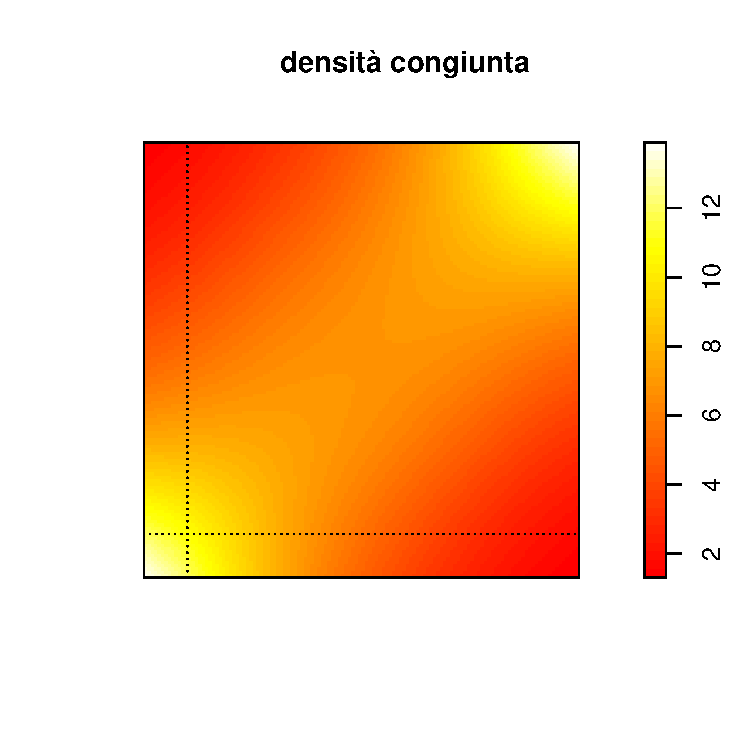
\includegraphics[width=0.5\textwidth]{plaatjes/bivaH0dep}
\end{center}

TODO: change plot

Remark: remember, however, that the marginal distributions are uniform because the two tests are under $H_0$.

\end{frame}




% \section{Bonferroni, Holm and Shaffer}
\section{Bonferroni (single-step)}


\bfr{Boole}
  \bb{Boolean inequality}
    Let two events $A$ e $B$:
    \[ \mathbb{P}(A \cup B) = \mathbb{P}(A) + \mathbb{P}(B) - \mathbb{P}(A \cap B) \]
    so
    \[ \mathbb{P}(A \cup B) \leq \mathbb{P}(A) + \mathbb{P}(B) \]
    Generalizing $A_1, \ldots, A_m$:
    \[ \mathbb{P}(\bigcup_{i=1}^m A_i) \leq \sum_{i=1}^m \mathbb{P}(A_i) \]
  \eb
  \bb{Equality}
    Equality occurs when events are disjointed
  \eb
  % \bb{Nessuna assumptione}
  %   Sempre valida
  % \eb
\end{frame}


\bfr{FamilyWise Error Rate (FWER)}
%\bb{Probability of doing AT LEAST one false rejection}
%  \eb


\bb{Bonferroni inequality}
     {Reduce $\alpha$} \\
    Reject $H_i$ if $p_i \leq \widetilde{\alpha} =\alpha/m$ ($m=$ number of hypotheses)
\eb
  \bb{FWER control}
    \begin{eqnarray*}
    \mathrm{FWER} &=& \mathbb{P} \big(p_i \leq \alpha/m\ \text{ for at least one $i$ true null hypothesis} \big) \\
    &=& \mathbb{P} \Big( \bigcup_{i\in \{\text{true null hypothesis}\}} \{p_i \leq \alpha/m\} \Big) \\
    &\leq& \sum_{i \in \{\text{true null hypothesis}\}} \mathbb{P} (p_i \leq \alpha/m) \\
    &\leq& m_0\frac{\alpha}{m} \leq m \frac{\alpha}{m}  = \alpha
    \end{eqnarray*}
  \eb
\end{frame}
% 
% 
% \bfr{The Bonferroni inequality}
%  \bb{Reduced $\alpha$}
%    Bonferroni: reduce significance level for each hypothesis
%    \\ Rifiuta $H_i$ if $p_i \leq \alpha/m$
%  \eb
%  \bb{Control of FWER}
%    \begin{eqnarray*}
%    \mathrm{FWER} &=& \mathrm{P} \big(\textrm{$p_i \leq \alpha/m$ for at least one $i$ with $H_i$ true} \big) \\
%    &=& \mathrm{P} \Big( \bigcup_{i\in T} \{p_i \leq \alpha/m\} \Big) \\
%    &\leq& \sum_{i \in T} \mathrm{P} (p_i \leq \alpha/m) \\
%    &\leq& \#T\frac{\alpha}{m} \leq \alpha
%    \end{eqnarray*}
%  \eb
% \end{frame}
% 


%%%%%%%%%%%%%%%%%BUONO PER MASTER, sostituiscono la successiva:
%%%%%%%%%%%%%%%%%BUONO PER MASTER, sostituiscono la successiva:
%%%%%%%%%%%%%%%%%BUONO PER MASTER, sostituiscono la successiva:
%%%%%%%%%%%%%%%%%BUONO PER MASTER, sostituiscono la successiva:
%%%%%%%%%%%%%%%%%BUONO PER MASTER, sostituiscono la successiva:
%%%%%%%%%%%%%%%%%BUONO PER MASTER, sostituiscono la successiva:
%%%%%%%%%%%%%%%%%BUONO PER MASTER, sostituiscono la successiva:
%%%%%%%%%%%%%%%%%BUONO PER MASTER, sostituiscono la successiva:
% \bfr{Using Bonferroni}
%  \bb{Advantages}
%    \bi
%      \item Extremely easy
%      \item Strong control of FWER under any dependence of p-values
%    \ei
%  \eb
%  \bb{Disadvantage}
%    Conservative: FWER $\leq \alpha$, often $<\alpha$
%  \eb
%  \bb{When is Bonferroni least conservative?}
%    \bi
%      \item Events $\{p_i \leq \alpha/m\}$ disjoint
%      \item $\# T = m$: complete null hypothesis
%    \ei
%  \eb
% \end{frame}
% 



\bfr{Bonferroni Procedure}

\bb{Multiplicity adjusted p-value}
$\tilde p_i = mp_i$ for $i=1,\ldots,m$ and reject if $\tilde p_i \leq \alpha$
\eb

\bb{Advantages}
\bi
\item Very simple
\item Controls the Family-Wise Error Rate (FWER) under any dependency
\ei
\eb

\bb{Disadvantages}
\bi
\item Conservative (Adjusted p-values are often high, leading to few rejections)
\ei
\eb
\end{frame}


\section{Holm (step-wise)}

\bfr{Holm's Procedure\footnote{Holm S. (1979) A simple sequentially rejective multiple test procedure. {\it Scandinavian Journal of Statistics}; 6(2):65--70.}}
%\textcolor{redUnipd}{$\quad$\textbf{Holm's sequential procedure}}

\begin{enumerate}
\item First step: adjusted p-value: $p\cdot m$; reject if $\leq \alpha$
\item After $r$ rejections, adjusted p-value: $p\cdot (m-r)$
\item Stop as soon as nothing is rejected
\end{enumerate}

\begin{center}
\begin{overprint}
\only<1>{\bbf{Bonferroni}}
\only<2>{\bbf{Suppose $p_A$ and $p_C$ are significant}}
\only<3>{\bbf{Adjusted p-value: $p\cdot 3$}}
\only<4>{\bbf{Suppose $p_D$ is significant}}
\only<5>{\bbf{Adjusted p-value: $p\cdot 2$}}
\only<6>{\bbf{No rejections. Stop}}
\begin{tikzpicture}
\node at (-.4,1) {$\mathcal{H}\setminus \mathcal{R}:$};
\node at (0,0) {$\mathcal{R}:$};
\node at (-1,2) {Adj. p-value:};
\node at (6,2) {\bbf{$\leq ? \alpha$}};
\only<1>{
\node at (1,2) {$p_A 5$};
\node at (2,2) {$p_B 5$};
\node at (3,2) {$p_C 5$};
\node at (4,2) {$p_D 5$};
\node at (5,2) {$p_E 5$};
\draw[] 
(1,1) node[draw, line width=1pt,fill=lightgrey] {A}
(2,1) node[draw, line width=1pt,fill=lightgrey] {B}
(3,1) node[draw, line width=1pt,fill=lightgrey] {C}
(4,1) node[draw, line width=1pt,fill=lightgrey] {D}
(5,1) node[draw, line width=1pt,fill=lightgrey] {E};}
\only<2>{
\node at (1,2) {$p_A 5$};
\node at (2,2) {$p_B 5$};
\node at (3,2) {$p_C 5$};
\node at (4,2) {$p_D 5$};
\node at (5,2) {$p_E 5$};
\draw[] 
(1,1) node[draw, line width=1pt,fill=lightred] {A}
(2,1) node[draw, line width=1pt,fill=lightgrey] {B}
(3,1) node[draw, line width=1pt,fill=lightred] {C}
(4,1) node[draw, line width=1pt,fill=lightgrey] {D}
(5,1) node[draw, line width=1pt,fill=lightgrey] {E};}
\only<3>{
\node at (1,2) {-};
\node at (2,2) {$p_B3$};
\node at (3,2) {-};
\node at (4,2) {$p_D3$};
\node at (5,2) {$p_E3$};
\draw[] 
(1,0) node[draw, line width=1pt,fill=lightred] {A}
(2,1) node[draw, line width=1pt,fill=lightgrey] {B}
(3,0) node[draw, line width=1pt,fill=lightred] {C}
(4,1) node[draw, line width=1pt,fill=lightgrey] {D}
(5,1) node[draw, line width=1pt,fill=lightgrey] {E};}
\only<4>{
\node at (1,2) {-};
\node at (2,2) {$p_B3$};
\node at (3,2) {-};
\node at (4,2) {$p_D3$};
\node at (5,2) {$p_E3$};
\draw[] 
(1,0) node[draw, line width=1pt,fill=lightred] {A}
(2,1) node[draw, line width=1pt,fill=lightgrey] {B}
(3,0) node[draw, line width=1pt,fill=lightred] {C}
(4,1) node[draw, line width=1pt,fill=lightred] {D}
(5,1) node[draw, line width=1pt,fill=lightgrey] {E};}
\only<5-6>{
\node at (1,2) {-};
\node at (2,2) {$p_B2$};
\node at (3,2) {-};
\node at (4,2) {-};
\node at (5,2) {$p_E2$};
\draw[] 
(1,0) node[draw, line width=1pt,fill=lightred] {A}
(2,1) node[draw, line width=1pt,fill=lightgrey] {B}
(3,0) node[draw, line width=1pt,fill=lightred] {C}
(4,0) node[draw, line width=1pt,fill=lightred] {D}
(5,1) node[draw, line width=1pt,fill=lightgrey] {E};}
\end{tikzpicture}
\end{overprint}
\end{center}
\end{frame}

\section{Closed Testing}
\begin{frame}{Union-intersection hypothesis}

Multiple testing problems in pharmaceutical applications are commonly formulated as \textbf{\rbf{union-intersection problems}}.

One rejects the global hypothesis of no effect if there is evidence of a positive effect with respect to \textbf{at least one} individual objective:

\begin{itemize}
    \item the trial's outcome is declared positive if at least one analysis produces a significant result,
    \item Each analysis is independently clinically relevant
    \item Each endpoint, dose, or population analysis independently provides proof of efficacy
\end{itemize}

Let denote the hypotheses $H_1, \dots, H_m$ corresponding to the multiple objectives. The hypotheses are tested against the alternative hypotheses $K_1, \dots, K_m$:
\begin{equation*}
    H_I: \cap_{i = 1}^m H_i \quad \text{versus} \quad H_U: \cup_{i=1}^m K_i
\end{equation*}

\bigskip

$\rightarrow$ adjust for multiplicity!

\end{frame}



\begin{frame}
\frametitle{Closed Testing\footnote{R Marcus, E Peritz, KR Gabriel (1976). On closed testing procedures with special reference to ordered analysis of variance. Biometrika 63: 655-660.}}
\begin{overprint}
\only<1>{Closed Set of Hypotheses (all possible intersections)}
\only<2>{Top Node Test (e.g., MANOVA)}
\only<9>{\bbf{Disadvantage: The tested hypotheses often become too many: $=2^{# \text{hypotheses}}-1$}}
\end{overprint}
\begin{center}
\only<1>{\bbf{Initial Hypotheses}}
\only<2>{\bbf{Closed Set}}
\only<3>{\bbf{Test the top node at level $\alpha$}}
\only<4>{\bbf{Suppose it is significant}}
\only<5>{\bbf{Move forward}}
\only<6>{\bbf{Check the next ones at level $\alpha$}}
\only<7>{\bbf{Move forward}}
\only<8-9>{\bbf{Identify the significant ones}}
\medskip

\begin{tikzpicture}
\only<1>{
\draw[] 
(0,4) node[draw, color=white] {A}
(-2,0) node[draw, line width=1pt] {A}
(0,0) node[draw, line width=1pt] {B}
(2,0) node[draw, line width=1pt] {C};
}
\only<2>{
\draw[] 
(0,4) node[draw, line width=1pt] {ABC}
(-1.5,2) node[draw, line width=1pt] {AB}
(0,2) node[draw, line width=1pt] {AC}
(1.5,2) node[draw, line width=1pt] {BC}
(-2,0) node[draw, line width=1pt] {A}
(0,0) node[draw, line width=1pt] {B}
(2,0) node[draw, line width=1pt] {C};
}
\only<3>{
\draw[] 
(.8,4) node {$\alpha$}
(0,4) node[draw, line width=1pt,fill=lightgrey] {ABC}
(-1.5,2) node[draw, line width=1pt] {AB}
(0,2) node[draw, line width=1pt] {AC}
(1.5,2) node[draw, line width=1pt] {BC}
(-2,0) node[draw, line width=1pt] {A}
(0,0) node[draw, line width=1pt] {B}
(2,0) node[draw, line width=1pt] {C};
}
\only<4>{
\draw[] 
(.8,4) node {-}
(0,4) node[draw, line width=1pt,fill=lightred] {ABC}
(-1.5,2) node[draw, line width=1pt] {AB}
(0,2) node[draw, line width=1pt] {AC}
(1.5,2) node[draw, line width=1pt] {BC}
(-2,0) node[draw, line width=1pt] {A}
(0,0) node[draw, line width=1pt] {B}
(2,0) node[draw, line width=1pt] {C};
}
\only<5>{
\draw[] 
(.8,4) node {-}
(2.1,2) node {$\alpha$}
(-.9,2) node {$\alpha$}
(.6,2) node {$\alpha$}
(0,4) node[draw, line width=1pt,fill=lightred] {ABC}
(-1.5,2) node[draw, line width=1pt,fill=lightgrey] {AB}
(0,2) node[draw, line width=1pt,fill=lightgrey] {AC}
(1.5,2) node[draw, line width=1pt,fill=lightgrey] {BC}
(-2,0) node[draw, line width=1pt] {A}
(0,0) node[draw, line width=1pt] {B}
(2,0) node[draw, line width=1pt] {C};
%\draw[->, line width=1pt] (0,3.7) -- (-1.5,2.3);
%\draw[->, line width=1pt] (0,3.7) -- (0,2.3);
%\draw[->, line width=1pt] (0,3.7) -- (1.5,2.3);
}
\only<6>{
\draw[] 
(.8,4) node {-}
(2.1,2) node {$\alpha$}
(-.9,2) node {-}
(.6,2) node {-}
(0,4) node[draw, line width=1pt,fill=lightred] {ABC}
(-1.5,2) node[draw, line width=1pt,fill=lightred] {AB}
(0,2) node[draw, line width=1pt,fill=lightred] {AC}
(1.5,2) node[draw, line width=1pt,fill=lightgrey] {BC}
(-2,0) node[draw, line width=1pt] {A}
(0,0) node[draw, line width=1pt] {B}
(2,0) node[draw, line width=1pt] {C};
%\draw[->, line width=1pt] (0,3.7) -- (-1.5,2.3);
%\draw[->, line width=1pt] (0,3.7) -- (0,2.3);
%\draw[->, line width=1pt] (0,3.7) -- (1.5,2.3);
}
\only<7>{
\draw[] 
(.8,4) node {-}
(2.1,2) node {$\alpha$}
(-.9,2) node {-}
(.6,2) node {-}
(-1.5,0) node {$\alpha$}
(0,4) node[draw, line width=1pt,fill=lightred] {ABC}
(-1.5,2) node[draw, line width=1pt,fill=lightred] {AB}
(0,2) node[draw, line width=1pt,fill=lightred] {AC}
(1.5,2) node[draw, line width=1pt,fill=lightgrey] {BC}
(-2,0) node[draw, line width=1pt,fill=lightgrey] {A}
(0,0) node[draw, line width=1pt] {B}
(2,0) node[draw, line width=1pt] {C};
%\draw[->, line width=1pt] (0,3.7) -- (-1.5,2.3);
%\draw[->, line width=1pt] (0,3.7) -- (0,2.3);
%\draw[->, line width=1pt] (0,3.7) -- (1.5,2.3);
%\draw[->, line width=1pt] (-1.5,1.7) -- (-2,0.3);
%\draw[->, line width=1pt] (0,1.7) -- (-1.7,0.3);
}
\only<8-9>{
\draw[] 
(.8,4) node {-}
(2.1,2) node {$\alpha$}
(-.9,2) node {-}
(.6,2) node {-}
(-1.5,0) node {-}
(0,4) node[draw, line width=1pt,fill=lightred] {ABC}
(-1.5,2) node[draw, line width=1pt,fill=lightred] {AB}
(0,2) node[draw, line width=1pt,fill=lightred] {AC}
(1.5,2) node[draw, line width=1pt,fill=lightgrey] {BC}
(-2,0) node[draw, line width=1pt,fill=lightred] {A}
(0,0) node[draw, line width=1pt] {B}
(2,0) node[draw, line width=1pt] {C};
%\draw[->, line width=1pt] (0,3.7) -- (-1.5,2.3);
%\draw[->, line width=1pt] (0,3.7) -- (0,2.3);
%\draw[->, line width=1pt] (0,3.7) -- (1.5,2.3);
%\draw[->, line width=1pt] (-1.5,1.7) -- (-2,0.3);
%\draw[->, line width=1pt] (0,1.7) -- (-1.7,0.3);
}
\end{tikzpicture}
\end{center}
\end{frame}

\section{Gatekeeping strategies}

\begin{frame}
\frametitle{Gatekeeping strategies}
Multiple objectives pursued in clinical trials typically exhibit a \textbf{hierarchical structure} $\rightarrow$ Primary and secondary objectives.

\bigskip

To construct a \textbf{gatekeeping procedure}, one first needs to define two or
more families of analyses, for example:
\begin{itemize}
    \item \rbf{Primary and secondary endpoints}: Primary endpoints determine the trial's outcome and key secondary endpoints provide useful supportive information about efficacy and safety
    \item \rbf{Primary and secondary populations}: General population versus subgroups of patients who are more likely to benefit from treatment
    \item \rbf{Primary and secondary tests}: Noninferiority assessment as the primary analysis followed by a superiority assessment
\end{itemize}


\end{frame}

\begin{frame}
\frametitle{Gatekeeping strategies}
\rbf{Family 1}:
$F_1 = \{H_1, \dots, H_{k_1}\}$, null hypotheses

$\dots$

\rbf{Family $m$}:
$F_m = \{H_{k_{m-1} +1}, \dots, H_{k_m}\}$, null hypotheses

\bigskip

Each family (except for the last one) serves as a \textbf{gatekeeper} for the next one, in the sense that one must pass it to perform analyses in the next family $\rightarrow$ increase power by accounting for \rbf{hierarchical} structure of multiple families.
\end{frame}

\begin{frame}
\frametitle{Gatekeeping Procedures}

\rbf{$\alpha$ recycling}

TODO: da mettere qui? spostare?

\begin{itemize}
    \item \textbf{Sequential Testing}: Families of hypotheses are tested sequentially starting with Family 1 $\rightarrow$ Error rate is transferred along the sequence
    \item \textbf{Sequential testing with re-testing}: Families of hypotheses are tested sequentially starting with Family 1 with a re-testing loop $\rightarrow$ Error rate is transferred along the sequence and then back to Family 1
    \item \textbf{Simultaneous testing}: Families of hypotheses are tested simultaneously $\rightarrow$ Error rate is transferred among families
\end{itemize}

    
\end{frame}

\begin{frame}
\frametitle{Gatekeeping Procedures}
\centering

\rbf{\textbf{Sequential Testing}}\\
\rbf{\textbf{(three ordered endpoints)}}

%\bigskip
\only<1>{\textcolor{cambridgedarkblue}{$\,$}}
\only<2>{\textcolor{cambridgedarkblue}{Start test A at $\alpha$}}
\only<3>{\textcolor{cambridgedarkblue}{Suppose $p_A<\alpha$}}
\only<4>{\textcolor{cambridgedarkblue}{Go on to test B at $\alpha$}}
\only<5>{\textcolor{cambridgedarkblue}{Suppose $p_B>\alpha$. Stop}}
\bigskip

\begin{tikzpicture}
% \draw[->, line width=1pt] (0,1.3) -- (0,0.7);
% \draw[->, line width=1pt] (0,3.3) -- (0,2.7);
\draw[] 
(1.3,4) node[color=white] {$\frac{\alpha}{2}$}
(-1.3,4) node[color=white] {$\frac{\alpha}{2}$};
\only<1>{
\draw[] 
(0,4) node[draw, line width=1pt, text width=1.7cm, text centered] {A\\ \small{primary endpoint}}
(0,2) node[draw, line width=1pt, text width=1.7cm, text centered] {B\\ \small{secondary endpoint}}
(0,0) node[draw, line width=1pt, text width=1.7cm, text centered] {C\\ \small{tertiary endpoint}};}
\only<2>{
\draw[] 
(1.3,4) node {$\alpha$}
(0,4) node[draw, line width=1pt, text width=1.7cm, text centered, fill=lightgrey] {A\\ \small{primary endpoint}}
(0,2) node[draw, line width=1pt, text width=1.7cm, text centered] {B\\ \small{secondary endpoint}}
(0,0) node[draw, line width=1pt, text width=1.7cm, text centered] {C\\ \small{tertiary endpoint}};}
\only<3>{
\draw[] 
(1.3,4) node {-}
(0,4) node[draw, line width=1pt, text width=1.7cm, text centered, fill=lightred]{A\\ \small{primary endpoint}}
(0,2) node[draw, line width=1pt, text width=1.7cm, text centered]{B\\ \small{secondary endpoint}}
(0,0) node[draw, line width=1pt, text width=1.7cm, text centered] {C\\ \small{tertiary endpoint}};}
\only<4>{
\draw[] 
(1.3,4) node {-}
(1.3,2) node {$\alpha$}
(0,4) node[draw, line width=1pt, text width=1.7cm, text centered, fill=lightred] {A\\ \small{primary endpoint}}(0,2) node[draw, line width=1pt, text width=1.7cm, text centered, fill=lightgrey] {B\\ \small{secondary endpoint}}
(0,0) node[draw, line width=1pt, text width=1.7cm, text centered] {C\\ \small{tertiary endpoint}};}
\only<5->{
\draw[] 
(1.3,4) node {-}
(1.3,2) node {$\alpha$}
(0,4) node[draw, line width=1pt, text width=1.7cm, text centered, fill=lightred] {A\\ \small{primary endpoint}}
(0,2) node[draw, line width=1pt, text width=1.7cm, text centered, fill=lightgrey] {B\\ \small{secondary endpoint}}
(0,0) node[draw, line width=1pt, text width=1.7cm, text centered] {C\\ \small{tertiary endpoint}};}
\end{tikzpicture}

\end{frame}
%%%%%%%%%%%%%%%%%%%%%%%%%%%%%%%%%%

\begin{frame}
\frametitle{Parallel Gatekeeping \footnote{Dmitrienko, A., Offen, W. W., and Westfall, P. H. (2003). Gatekeeping strategies for clinical trials that do not require all primary effects to be significant. Statistics in medicine, 22(15), 2387-2400.}}

Family $1$ is a \rbf{parallel gatekeeper} for Family $2$, i.e., at least one hypothesis must be rejected in Family $1$ to proceed to Family $2$.

\bigskip

\rbf{\textbf{Example}}: Schizophrenia trial

\textbf{Objective}: Evaluate the efficacy of a treatment in patients diagnosed with schizophrenia

\textbf{Design}: Two doses of treatment (Doses L and H) versus placebo. Treatment effect on at least one dose must be
significant.

\textbf{Primary endpoint}: Positive and Negative Symptoms Scale (PANSS) total score

\textbf{Two patient populations}: General population and subpopulation (based on a genotypic classifier)
\end{frame}


\begin{frame}
\frametitle{Parallel Gatekeeping}
\definecolor{lightred}{RGB}{255, 179, 178}
\tikzstyle{comp1} = [draw, rectangle, rounded corners, minimum height=1cm, minimum width=2cm, fill=lightred]

\tikzstyle{arrow} = [thick,->,>=stealth]

\begin{figure}
\centering

\begin{tikzpicture}[node distance=2.2cm]
%%% NODES %%%
\node (main1)     [comp1]                 {$H_1$};
\node (main2)     [comp1, right of=main1]                 {$H_2$};

\node (text1)        [left of=main]     {\hspace{-5cm} \textbf{Family 1} };
\node (s1)         [comp1, below of=main1]      {$H_3$};
\node (s2)        [comp1, below of=main2]     {$H_4$};

\node (text2) [below of=text1]     {\hspace{-5cm}\textbf{Family 2}};
%%% ARROWS %%%
\draw [arrow] (main1) -- (s1);
\draw [arrow] (main1) -- (s2);
\draw [arrow] (main2) -- (s1);
\draw [arrow] (main2) -- (s2);
\end{tikzpicture}
\end{figure}
\bigskip

\textbf{Family 1}: $\{H_1, H_2\}$ Doses L and H versus Placebo in overall population

\textbf{Family 2}: $\{H_3, H_4\}$ Doses L and H versus Placebo in subpopulation
\end{frame}

\begin{frame}
\frametitle{Parallel Gatekeeping}

\centering

\bigskip
% \only<1-5>{\textcolor{cambridgedarkblue}{$\,$ }}
\only<1>{\textcolor{cambridgedarkblue}{Start test $H_1$ and $H_2$ at $\alpha/2$}}
\only<2>{\textcolor{cambridgedarkblue}{Suppose $p_1< \alpha/2$}}
\only<3>{\textcolor{cambridgedarkblue}{Test $H_3$ and $H_4$ at $\alpha/4$}}
\only<4>{\textcolor{cambridgedarkblue}{Suppose $p_4< \alpha/4$}}
\only<5>{\textcolor{cambridgedarkblue}{Test $H_3$ at $\alpha/2$}}
\only<6>{\textcolor{cambridgedarkblue}{Suppose $p_3<\alpha/2$}}
\only<7>{\textcolor{cambridgedarkblue}{Test $H_2$ at $\alpha$}}
\bigskip

\begin{tikzpicture}
\draw[] 
(4.3,2.8) node[color=white] {$\frac{\alpha}{2}$}
(-1.3,2.8) node[color=white] {$\frac{\alpha}{2}$};
\only<1>{\draw[] 
(0,2.8) node[draw, line width=1pt, text width=1.9cm, text centered, fill=lightgrey] {$H_1$ Dose L \\ \small{overall population}}
(-1.3,2.8) node {$\frac{\alpha}{2}$}
(3,2.8) node[draw, line width=1pt, text width=1.9cm, text centered, fill=lightgrey] {$H_2$ Dose H \\ \small{overall population}}
(4.3,2.8) node {$\frac{\alpha}{2}$}
(0,0.2) node[draw, line width=1pt, text width=1.9cm, text centered] {$H_3$ Dose L \\ \small{sub-population}}
(3,0.2) node[draw, line width=1pt, text width=1.9cm, text centered] {$H_4$ Dose H \\ \small{sub-population}};}
\only<2>{\draw[] 
(-1.3,2.8) node {-}
(4.3,2.8) node {$\frac{\alpha}{2}$}
(0,2.8) node[draw, line width=1pt, text width=1.9cm, text centered, fill=lightred] {$H_1$ Dose L \\ \small{overall population}}
(3,2.8) node[draw, line width=1pt, text width=1.9cm, text centered, fill=lightgrey] {$H_2$ Dose H \\ \small{overall population}}
(0,0.2) node[draw, line width=1pt, text width=1.9cm, text centered] {$H_3$ Dose L \\ \small{sub-population}}
(3,0.2) node[draw, line width=1pt, text width=1.9cm, text centered] {$H_4$ Dose H \\ \small{sub-population}};}
\only<3>{\draw[] 
(-1.3,2.8) node {-}
(4.3,2.8) node {$\frac{\alpha}{2}$}
(4.3,0.2) node {$\frac{\alpha}{4}$}
(-1.3,0.2) node {$\frac{\alpha}{4}$}
(0,2.8) node[draw, line width=1pt, text width=1.9cm, text centered, fill=lightred] {$H_1$ Dose L \\ \small{overall population}}
(3,2.8) node[draw, line width=1pt, text width=1.9cm, text centered, fill=lightgrey] {$H_2$ Dose H \\ \small{overall population}}
(0,0.2) node[draw, line width=1pt, text width=1.9cm, text centered, fill=lightgrey] {$H_3$ Dose L \\ \small{sub-population}}
(3,0.2) node[draw, line width=1pt, text width=1.9cm, text centered, fill=lightgrey] {$H_4$ Dose H \\ \small{sub-population}};}
\only<4>{\draw[] 
(-1.3,2.8) node {-}
(4.3,2.8) node {$\frac{\alpha}{2}$}
(4.3,0.2) node {-}
(-1.3,0.2) node {$\frac{\alpha}{4}$}
(0,2.8) node[draw, line width=1pt, text width=1.9cm, text centered, fill=lightred] {$H_1$ Dose L \\ \small{overall population}}
(3,2.8) node[draw, line width=1pt, text width=1.9cm, text centered, fill=lightgrey] {$H_2$ Dose H \\ \small{overall population}}
(0,0.2) node[draw, line width=1pt, text width=1.9cm, text centered, fill=lightgrey] {$H_3$ Dose L \\ \small{sub-population}}
(3,0.2) node[draw, line width=1pt, text width=1.9cm, text centered, fill=lightred] {$H_4$ Dose H \\ \small{sub-population}};}
\only<5>{\draw[] 
(-1.3,2.8) node {-}
(4.3,2.8) node {$\frac{\alpha}{2}$}
(4.3,0.2) node {-}
(-1.3,0.2) node {$\frac{\alpha}{2}$}
(0,2.8) node[draw, line width=1pt, text width=1.9cm, text centered, fill=lightred] {$H_1$ Dose L \\ \small{overall population}}
(3,2.8) node[draw, line width=1pt, text width=1.9cm, text centered, fill=lightgrey] {$H_2$ Dose H \\ \small{overall population}}
(0,0.2) node[draw, line width=1pt, text width=1.9cm, text centered, fill=lightgrey] {$H_3$ Dose L \\ \small{sub-population}}
(3,0.2) node[draw, line width=1pt, text width=1.9cm, text centered, fill=lightred] {$H_4$ Dose H \\ \small{sub-population}};}
\only<6>{\draw[] 
(-1.3,2.8) node {-}
(4.3,0.2) node {-}
(-1.3,0.2) node {-}
(4.3,2.8) node {$\frac{\alpha}{2}$}
(0,2.8) node[draw, line width=1pt, text width=1.9cm, text centered, fill=lightred] {$H_1$ Dose L \\ \small{overall population}}
(3,2.8) node[draw, line width=1pt, text width=1.9cm, text centered, fill=lightgrey] {$H_2$ Dose H \\ \small{overall population}}
(0,0.2) node[draw, line width=1pt, text width=1.9cm, text centered, fill=lightred] {$H_3$ Dose L \\ \small{sub-population}}
(3,0.2) node[draw, line width=1pt, text width=1.9cm, text centered, fill=lightred] {$H_4$ Dose H \\ \small{sub-population}};}
\only<7>{\draw[] 
(-1.3,2.8) node {-}
(4.3,0.2) node {-}
(-1.3,0.2) node {-}
(4.3,2.8) node {$\alpha$}
(0,2.8) node[draw, line width=1pt, text width=1.9cm, text centered, fill=lightred] {$H_1$ Dose L \\ \small{overall population}}
(3,2.8) node[draw, line width=1pt, text width=1.9cm, text centered, fill=lightgrey] {$H_2$ Dose H \\ \small{overall population}}
(0,0.2) node[draw, line width=1pt, text width=1.9cm, text centered, fill=lightred] {$H_3$ Dose L \\ \small{sub-population}}
(3,0.2) node[draw, line width=1pt, text width=1.9cm, text centered, fill=lightred] {$H_4$ Dose H \\ \small{sub-population}};}
\end{tikzpicture}

\bigskip

secondary endpoints are tested if at least one
primary test is significant


% \end{columns}

\end{frame}

\begin{frame}
\frametitle{Parallel Gatekeeping}
\begin{overprint}
  \onslide<1>
    Test all primary endpoints at $\alpha/3$
  \onslide<2>
    If we reject a few\ldots
  \onslide<3>
    Go on with the other primary endpoints as in Holm's procedure
  \onslide<4>
    Suppose we are able to reject all primary endpoints\ldots
  \onslide<5>
    Go on testing the secondary endpoints at $\alpha/3$
  \onslide<6>
    And if we reject some of those\ldots
  \onslide<7>
    Go on doing Holm for the secondary endpoints
\end{overprint}
\begin{figure}
  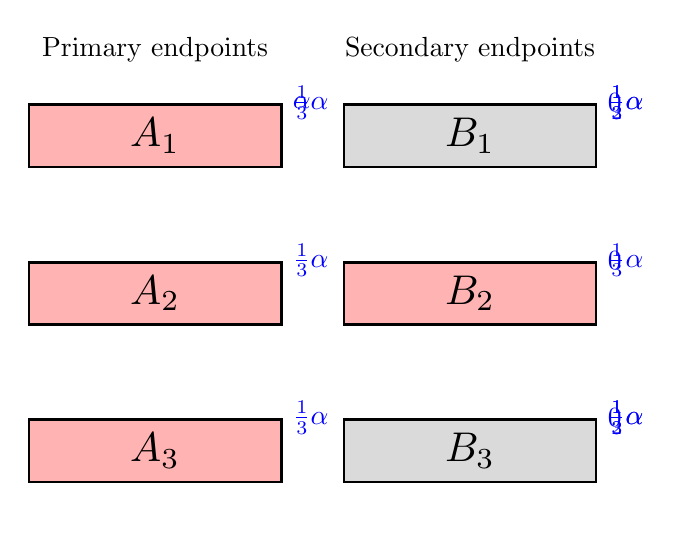
\begin{tikzpicture}
  \path (0,0) rectangle (7,6) ;
  \path<1-3> (1,5) node[draw, scale=1.5,  line width=1pt, text width=1.9cm, text centered, fill=lightgrey] (a1) {$A_1$} ;
  \path<4-> (1,5) node[draw, scale=1.5, line width=1pt, text width=1.9cm, text centered, fill=lightred] (a1) {$A_1$} ;
  \path<1-2> (a1.north east) node[anchor=west, blue] {$\frac13\alpha$} ;
  \path<3> (a1.north east) node[anchor=west, blue] {$\alpha$} ;

  \path<1> (1,3) node[draw, scale=1.5,  line width=1pt, text width=1.9cm, text centered, fill=lightgrey] (a2) {$A_2$} ;
  \path<2-> (1,3) node[draw, scale=1.5, line width=1pt, text width=1.9cm, text centered, fill=lightred] (a2) {$A_2$} ;
  \path<1> (a2.north east) node[anchor=west, blue] {$\frac13\alpha$} ;

  \path<1> (1,1) node[draw, scale=1.5,  line width=1pt, text width=1.9cm, text centered, fill=lightgrey] (a3) {$A_3$} ;
  \path<2-> (1,1) node[draw, scale=1.5, line width=1pt, text width=1.9cm, text centered, fill=lightred] (a3) {$A_3$} ;
  \path<1> (a3.north east) node[anchor=west, blue] {$\frac13\alpha$} ;

  \path<1-4> (5,5) node[draw, scale=1.5,  line width=1pt, text width=1.9cm, text centered] (b1) {$B_1$} ;
  \path<5-> (5,5) node[draw, scale=1.5,  line width=1pt, text width=1.9cm, text centered, fill=lightgrey] (b1) {$B_1$} ;
  \path<1-4> (b1.north east) node[anchor=west, blue] {$0$} ;
  \path<5-6> (b1.north east) node[anchor=west, blue] {$\frac13\alpha$} ;
  \path<7-> (b1.north east) node[anchor=west, blue] {$\frac12\alpha$} ;

  \path<1-4> (5,3) node[draw, scale=1.5,  line width=1pt, text width=1.9cm, text centered] (b2) {$B_2$} ;
  \path<5> (5,3) node[draw, scale=1.5,  line width=1pt, text width=1.9cm, text centered, fill=lightgrey] (b2) {$B_2$} ;
  \path<6-> (5,3) node[draw, scale=1.5, line width=1pt, text width=1.9cm, text centered, fill=lightred] (b2) {$B_2$} ;
  \path<1-4> (b2.north east) node[anchor=west, blue] {$0$} ;
  \path<5> (b2.north east) node[anchor=west, blue] {$\frac13\alpha$} ;

  \path<1-4> (5,1) node[draw, scale=1.5,  line width=1pt, text width=1.9cm, text centered] (b3) {$B_3$} ;
  \path<5-> (5,1) node[draw, scale=1.5,  line width=1pt, text width=1.9cm, text centered, fill=lightgrey] (b3) {$B_3$} ;
  \path<1-4> (b3.north east) node[anchor=west, blue] {$0$} ;
  \path<5-6> (b3.north east) node[anchor=west, blue] {$\frac13\alpha$} ;
  \path<7-> (b3.north east) node[anchor=west, blue] {$\frac12\alpha$} ;

  \path (1,6.1) node {Primary endpoints} ;
  \path (5,6.1) node {Secondary endpoints} ;
  \end{tikzpicture}
\end{figure}
\end{frame}


\begin{frame}
\frametitle{Parallel Gatekeeping}
\begin{overprint}
  \onslide<1>
    Test all primary endpoints at $\alpha/3$
  \onslide<2>
    If we reject a few\ldots
  \onslide<3>
    Go on with the secondary endpoints with the available $\alpha$
  \onslide<4>
    Suppose we are able to reject some of the secondary endpoints\ldots
  \onslide<5>
    Go on doing Holm for the secondary endpoints
  \onslide<6>
    And if we reject all secondary ones\ldots
  \onslide<7>
    Go on doing Holm for the primary endpoints
\end{overprint}
\begin{figure}
  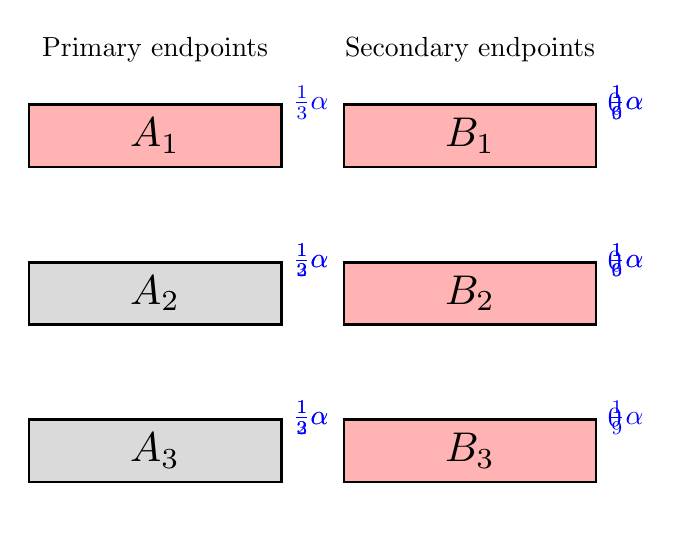
\begin{tikzpicture}
  \path (0,0) rectangle (7,6) ;
  \path<1> (1,5) node[draw, scale=1.5,  line width=1pt, text width=1.9cm, text centered, fill=lightgrey] (a1) {$A_1$} ;
  \path<2-> (1,5) node[draw, scale=1.5, line width=1pt, text width=1.9cm, text centered, fill=lightred] (a1) {$A_1$} ;
  \path<1> (a1.north east) node[anchor=west, blue] {$\frac13\alpha$} ;

  \path (1,3) node[draw, scale=1.5,  line width=1pt, text width=1.9cm, text centered, fill=lightgrey] (a2) {$A_2$} ;
  \path<1-6> (a2.north east) node[anchor=west, blue] {$\frac13\alpha$} ;
  \path<7-> (a2.north east) node[anchor=west, blue] {$\frac12\alpha$} ;

  \path (1,1) node[draw, scale=1.5,  line width=1pt, text width=1.9cm, text centered, fill=lightgrey] (a3) {$A_3$} ;
  \path<1-6> (a3.north east) node[anchor=west, blue] {$\frac13\alpha$} ;
  \path<7-> (a3.north east) node[anchor=west, blue] {$\frac12\alpha$} ;

  \path<1-2> (5,5) node[draw, scale=1.5,  line width=1pt, text width=1.9cm, text centered] (b1) {$B_1$} ;
  \path<3-5> (5,5) node[draw, scale=1.5,  line width=1pt, text width=1.9cm, text centered, fill=lightgrey] (b1) {$B_1$} ;
  \path<6-> (5,5) node[draw, scale=1.5, line width=1pt, text width=1.9cm, text centered, fill=lightred] (b1) {$B_1$} ;
  \path<1-2> (b1.north east) node[anchor=west, blue] {$0$} ;
  \path<3-4> (b1.north east) node[anchor=west, blue] {$\frac19\alpha$} ;
  \path<5> (b1.north east) node[anchor=west, blue] {$\frac16\alpha$} ;

  \path<1-2> (5,3) node[draw, scale=1.5,  line width=1pt, text width=1.9cm, text centered] (b2) {$B_2$} ;
  \path<3-5> (5,3) node[draw, scale=1.5,  line width=1pt, text width=1.9cm, text centered, fill=lightgrey] (b2) {$B_2$} ;
  \path<6-> (5,3) node[draw, scale=1.5, line width=1pt, text width=1.9cm, text centered, fill=lightred] (b2) {$B_2$} ;
  \path<1-2> (b2.north east) node[anchor=west, blue] {$0$} ;
  \path<3-4> (b2.north east) node[anchor=west, blue] {$\frac19\alpha$} ;
  \path<5> (b2.north east) node[anchor=west, blue] {$\frac16\alpha$} ;

  \path<1-2> (5,1) node[draw, scale=1.5,  line width=1pt, text width=1.9cm, text centered ] (b3) {$B_3$} ;
  \path<3> (5,1) node[draw, scale=1.5,  line width=1pt, text width=1.9cm, text centered, fill=lightgrey] (b3) {$B_3$} ;
  \path<4-> (5,1) node[draw, scale=1.5, line width=1pt, text width=1.9cm, text centered, fill=lightred] (b3) {$B_3$} ;
  \path<1-2> (b3.north east) node[anchor=west, blue] {$0$} ;
  \path<3> (b3.north east) node[anchor=west, blue] {$\frac19\alpha$} ;

  \path (1,6.1) node {Primary endpoints} ;
  \path (5,6.1) node {Secondary endpoints} ;
  \end{tikzpicture}
\end{figure}
\end{frame}

\begin{frame}
\frametitle{Intersection-Union test}

Intersection-union testing arises naturally in studies when a significant outcome with respect to two or more objectives is required in order to declare the study successful.

\begin{itemize}
    \item All analyses must show benefit
    \item The trial's outcome is positive if all analyses
produce a significant outcome
\end{itemize}

\begin{equation*}
    H_I: \cup_{i = 1}^m H_i \quad \text{versus} H_U: \cap_{i=1}^m K_i
\end{equation*}

\bigskip

$\rightarrow$ no multiplicity adjustment. 

    
\end{frame}

\begin{frame}
\frametitle{Serial Gatekeeping \footnote{Westfall, P. H., & Krishen, A. (2001). Optimally weighted, fixed sequence and gatekeeper multiple testing procedures. Journal of Statistical Planning and Inference, 99(1), 25-40.}}

Family $1$ is a \rbf{serial gatekeeper} for Family $2$ $\rightarrow$ all hypotheses must be rejected in Family $1$ to proceed to Family $2$.

\bigskip
\rbf{\textbf{Example}}: Alzheimer's diseases trial

\textbf{Objective}: Evaluate the effects of a treatment on cognition
and global changes in patients with mild to moderate Alzheimer's disease

\textbf{Design}: Treatment versus placebo

\textbf{Primary endpoints}: Endpoint 1: Cognition endpoint (ADAS-Cog), Endpoint 2: Clinical global scale (CIBIC plus)

Treatment effect on both endpoints must be significant

\textbf{Secondary endpoints}; Endpoint 3: Biochemical marker, Endpoint 4: Imaging marker
\end{frame}

\begin{frame}
\frametitle{Serial Gatekeeping}
\tikzstyle{comp1} = [draw, rectangle, rounded corners, minimum height=1cm, minimum width=4cm, fill=lightred]
\tikzstyle{comp2} = [draw, rectangle, rounded corners, minimum height=1cm, minimum width=2cm, fill=lightred]
\tikzstyle{arrow} = [thick,->,>=stealth]

\begin{figure}
\centering

\begin{tikzpicture}[node distance=2.2cm]
%%% NODES %%%
\node (main)     [comp1]                 {$H_1$ and $H_2$};
\node (text1)        [left of=main]     {\hspace{-5cm} \textbf{Family 1} };
\coordinate[below of=main] (c);
\node (s1)         [comp2, left of=c]      {$H_3$};
\node (s2)        [comp2, right of=c]     {$H_4$};

\node (text2) [below of=text1]     {\hspace{-5cm}\textbf{Family 2}};
%%% ARROWS %%%
\draw [arrow] (main) -- (s1);
\draw [arrow] (main) -- (s2);
\end{tikzpicture}
\end{figure}
\textbf{Family 1}: $\{H_1, H_2\}$  Treatment versus Placebo on cognition and clinical global scale

\textbf{Family 2}: $\{H_3, H_4\}$  Treatment versus Placebo on biochemical and imaging marker
\end{frame}

\begin{frame}
\frametitle{Serial Gatekeeping}

\centering

\bigskip
% \only<1-5>{\textcolor{cambridgedarkblue}{$\,$ }}
\only<1>{\textcolor{cambridgedarkblue}{Start test $H_1$ and $H_2$ at $\alpha$}}
\only<2>{\textcolor{cambridgedarkblue}{Suppose $p_1< \alpha$ and $p_2 < \alpha$}}
\only<3>{\textcolor{cambridgedarkblue}{Test $H_3$ at $\alpha/2$}}
\only<4>{\textcolor{cambridgedarkblue}{Suppose $p_3< \alpha/2$}}
\only<5>{\textcolor{cambridgedarkblue}{Test $H_4$ at $\alpha$}}
\bigskip

\begin{tikzpicture}
\draw[] 
(4.3,2.8) node[color=white] {$\frac{\alpha}{2}$}
(-1.3,2.8) node[color=white] {$\frac{\alpha}{2}$};
\only<1>{\draw[] 
(0,2.8) node[draw, line width=1pt, text width=1.9cm, text centered, fill=lightgrey] {$H_1$ Treatment \\ \small{cognition}}
(-1.3,2.8) node {$\alpha$}
(3,2.8) node[draw, line width=1pt, text width=1.9cm, text centered, fill=lightgrey] {$H_2$ Treatment \\ \small{clinical global scale}}
(4.3,2.8) node {$\alpha$}
(0,0.2) node[draw, line width=1pt, text width=1.9cm, text centered] {$H_3$ Treatment \\ \small{biochemical marker}}
(3,0.2) node[draw, line width=1pt, text width=1.9cm, text centered] {$H_4$ Treatment \\ \small{imaging marker}};}
\only<2>{\draw[] 
(-1.3,2.8) node {-}
(4.3,2.8) node {-}
(0,2.8) node[draw, line width=1pt, text width=1.9cm, text centered, fill=lightred] {$H_1$ Treatment \\ \small{cognition}}
(3,2.8) node[draw, line width=1pt, text width=1.9cm, text centered, fill=lightred] {$H_2$ Treatment \\ \small{clinical global scale}}
(0,0.2) node[draw, line width=1pt, text width=1.9cm, text centered] {$H_3$ Treatment \\ \small{biochemical marker}}
(3,0.2) node[draw, line width=1pt, text width=1.9cm, text centered] {$H_4$ Treatment \\ \small{imaging marker}};}
\only<3>{\draw[] 
(-1.3,2.8) node {-}
(4.3,2.8) node {-}
(4.3,0.2) node {-}
(-1.3,0.2) node {$\frac{\alpha}{2}$}
(0,2.8) node[draw, line width=1pt, text width=1.9cm, text centered, fill=lightred] {$H_1$ Treatment \\ \small{cognition}}
(3,2.8) node[draw, line width=1pt, text width=1.9cm, text centered, fill=lightred] {$H_2$ Treatment \\ \small{clinical global scale}}
(0,0.2) node[draw, line width=1pt, text width=1.9cm, text centered, fill=lightgrey] {$H_3$ Treatment \\ \small{biochemical marker}}
(3,0.2) node[draw, line width=1pt, text width=1.9cm, text centered, fill=white] {$H_4$ Treatment \\ \small{imaging marker}};}
\only<4>{\draw[] 
(-1.3,2.8) node {-}
(4.3,2.8) node {-}
(4.3,0.2) node {-}
(-1.3,0.2) node {-}
(0,2.8) node[draw, line width=1pt, text width=1.9cm, text centered, fill=lightred] {$H_1$ Treatment \\ \small{cognition}}
(3,2.8) node[draw, line width=1pt, text width=1.9cm, text centered, fill=lightred] {$H_2$ Treatment \\ \small{clinical global scale}}
(0,0.2) node[draw, line width=1pt, text width=1.9cm, text centered, fill=lightred] {$H_3$ Treatment \\ \small{biochemical marker}}
(3,0.2) node[draw, line width=1pt, text width=1.9cm, text centered, fill=white] {$H_4$ Treatment \\ \small{imaging marker}};}
\only<5>{\draw[] 
(-1.3,2.8) node {-}
(4.3,2.8) node {-}
(4.3,0.2) node {$\alpha$}
(-1.3,0.2) node {-}
(0,2.8) node[draw, line width=1pt, text width=1.9cm, text centered, fill=lightred] {$H_1$ Treatment \\ \small{cognition}}
(3,2.8) node[draw, line width=1pt, text width=1.9cm, text centered, fill=lightred] {$H_2$ Treatment \\ \small{clinical global scale}}
(0,0.2) node[draw, line width=1pt, text width=1.9cm, text centered, fill=lightred] {$H_3$ Treatment \\ \small{biochemical marker}}
(3,0.2) node[draw, line width=1pt, text width=1.9cm, text centered, fill=lightgrey] {$H_4$ Treatment \\ \small{imaging marker}};}

\end{tikzpicture}

\bigskip

secondary endpoints are tested if all primary tests are significant


% \end{columns}

\end{frame}





\section{Summary}
\bfr{Summary}
\bb{Family-Wise Error}
\bi
\item Generalizes Type I errors to the case of multiple hypotheses
\pause
\item Controls the probability of \textbf{at least one} false rejection among all rejections
\pause
\item Adjusts p-values (adjusted p-values are always equal to or worse than the unadjusted p-values)
\pause
\item Understand the hierarchical/sequential structure of hypotheses testing $\rightarrow$ increase power
\ei
\eb
\pause
\bb{R Software}
\bi
\item Bonferroni and Holm: {\tt library(stats); p.adjust()}
\item Closed Testing: {\tt library(cherry); closed()}
% \item Structured Hypotheses: {\tt library(globaltest); inheritance()}
\item Post-hoc and more: {\tt library(multcomp); glht()}
% \item Permutations - Westfall \&\ Young: {\tt library(flip); flip.adjust()}
\ei
\eb
\end{frame}
%%%%%%%%%%%%%%%%%%%%%

\end{document}


